\documentclass[11pt,a4paper]{article}

% --- Packages ---------------------------------------------------------------
\usepackage[utf8]{inputenc}
\usepackage[T1]{fontenc}
\usepackage{lmodern}
\usepackage[margin=2.5cm]{geometry}
\usepackage{graphicx}
\usepackage{booktabs}
\usepackage{amsmath, amssymb}
\usepackage{hyperref}
\usepackage{xcolor}
\usepackage{caption}
\usepackage{subcaption}
\usepackage{listings}
\usepackage{authblk}
\usepackage{enumitem}

\hypersetup{
    colorlinks=true,
    linkcolor=blue!50!black,
    citecolor=blue!50!black,
    urlcolor=blue!70!black,
}

% Code listing style
\definecolor{codebg}{HTML}{F7F7F7}
\lstset{
    backgroundcolor=\color{codebg},
    basicstyle=\ttfamily\small,
    breaklines=true,
    frame=single,
    numbers=left,
    numberstyle=\tiny\color{gray},
}

% --- Front matter -----------------------------------------------------------
\title{
    \textbf{Project Omni-Arb}\\[0.4em]
    \large An ML-Gated Triangular Arbitrage System for Crypto Spot Markets:\\
    Architecture, Empirical Evidence, and Limits
}
\author{
    Andrea Cammarano \quad Giacomo Lanni \quad Edoardo Praderio \\
    \small Università della Svizzera italiana --- Master in Finance \\
    \small Corresponding author: \texttt{edoardo.praderio23@gmail.com}
}
\date{\today}

\begin{document}
\maketitle

% ---------------------------------------------------------------------------
\begin{abstract}
We design, implement, and empirically evaluate a triangular arbitrage system for crypto spot markets, spanning four major exchanges (Binance, Bybit, Coinbase, Kraken) and three currencies (USDT, BTC, ETH). The system is structured around a \emph{Triple-Gate} decision pipeline: (i) a Bellman--Ford profit gate that filters cycles by post-fee log-return, (ii) a LightGBM \emph{Guardian} ML model that scores cycles by their conditional probability of pre-fee profitability, and (iii) a Sentinel risk module that enforces inventory and drawdown constraints. Over 9.6 million order-book snapshots and 5{,}560 candidate cycles recorded across all four venues, we find that (a) pre-fee triangular mispricings are pervasive, occurring in 16.8\% of tick-level observations; (b) realistic retail taker fees of 10--60 basis points per leg consume all such opportunities, producing zero positive-EV trades in our 2-day sample; (c) the Guardian achieves an out-of-sample AUC of 0.61 and improves the hit rate of selected cycles by +4 percentage points over random selection (23.0\% vs.\ 19.0\%); and (d) under a frictionless-execution counterfactual, the methodology produces measurably better-than-random risk-adjusted returns, demonstrating the architecture is sound even though current market microstructure does not support a profitable production deployment at retail-fee tiers.
\end{abstract}

% ---------------------------------------------------------------------------
\section{Introduction}

% [INSTRUCTOR-FRIENDLY MOTIVATION: replace with your own framing in 2-3 paragraphs.]
Triangular arbitrage --- the simultaneous execution of three sequential currency conversions that returns more of the starting currency than was committed --- is a textbook no-arbitrage condition in foreign-exchange markets. In crypto spot markets, where venues vary widely in liquidity, fee schedule, and microstructure, the question of whether \emph{exploitable} triangular cycles exist is empirical rather than theoretical. This project addresses that question end-to-end: from continuous data collection, through detection and classification, to backtest evaluation.

We make four contributions:
\begin{enumerate}[label=(\roman*)]
    \item A reproducible data pipeline that streams real-time order-book snapshots from four exchanges into PostgreSQL via CCXT Pro WebSockets.
    \item A Bellman--Ford negative-cycle detector with venue-specific fee accounting, enumerating both rotations of the USDT-BTC-ETH triangle per venue per poll.
    \item A walk-forward-validated LightGBM classifier (\emph{Guardian}) that predicts pre-fee cycle profitability from venue, direction, time-of-day, and rolling-momentum features.
    \item A three-scenario backtest (realistic, maker rebate, frictionless) that quantifies the fee elasticity of the strategy's expected value.
\end{enumerate}

The remainder of the paper is organised as follows. Section~\ref{sec:background} reviews triangular arbitrage and crypto market microstructure. Section~\ref{sec:architecture} describes the Triple-Gate architecture. Section~\ref{sec:data} reports data-collection methodology. Section~\ref{sec:methods} details the detection algorithm, feature engineering, and training procedure. Section~\ref{sec:results} presents results. Section~\ref{sec:discussion} interprets findings and discusses limitations. Section~\ref{sec:conclusion} concludes.

% ---------------------------------------------------------------------------
\section{Background}
\label{sec:background}

\subsection{Triangular arbitrage}
A triangular cycle consists of three sequential trades $C_0 \to C_1 \to C_2 \to C_0$ that returns the strategy to its starting currency $C_0$. Letting $r_{ij}$ denote the effective exchange rate of $C_i \to C_j$ after taker fees $\phi_i \in [0,1)$, the cycle is profitable iff
\begin{equation}
\prod_{k=0}^{2} r_{k,k+1\,(\!\!\bmod 3)} (1 - \phi) > 1,
\end{equation}
or equivalently, in log-space,
\begin{equation}
\sum_{k=0}^{2} \ln\!\Big( r_{k,k+1\,(\!\!\bmod 3)} (1 - \phi) \Big) > 0.
\end{equation}

This logarithmic transformation is what permits us to cast triangular-arbitrage detection as a shortest-path negative-cycle problem on a graph whose edge weights are $w_{ij} = -\ln(r_{ij}(1-\phi))$.

\subsection{The fee structure as binding constraint}
Crypto exchanges charge per-leg taker fees ranging from approximately $\phi = 10$ bps (Binance, Bybit) to $\phi = 60$ bps (Coinbase) at retail tiers, with maker rebates available to high-volume accounts. A three-leg cycle therefore incurs cumulative fees of $3\phi \in [30, 180]$ bps. For pre-fee mispricings between major USDT pairs typically observed at 1--15 bps, the fee structure represents a binding economic constraint, as we empirically confirm in Section~\ref{sec:results}.

% ---------------------------------------------------------------------------
\section{System Architecture}
\label{sec:architecture}

The system implements a five-component pipeline. Figure~\ref{fig:architecture} (omitted in this draft) presents the dataflow diagram.

\paragraph{Scout.} A unified CCXT Pro WebSocket streamer subscribes simultaneously to depth-10 (Kraken) and depth-50 (Bybit spot) order books for BTC/USDT, ETH/USDT, and ETH/BTC across all four venues. Each tick is persisted via psycopg2 to a \texttt{book\_snapshots} Postgres table, with offload to a worker thread so the WebSocket loop is never blocked on database I/O.

\paragraph{Brain.} A source-free Bellman--Ford algorithm with fee-aware edge weights $w_{ij} = -\ln(r_{ij}(1-\phi))$ detects negative cycles. We enumerate both rotations of the canonical USDT-BTC-ETH triangle per venue per poll (Section~\ref{sec:methods}), producing 8 candidate cycles per 2-second poll across all venues.

\paragraph{Profit Gate (Gate 1).} Implements a tunable post-fee log-return threshold (default 5 bps). Rejects cycles whose net expected return does not clear the buffer.

\paragraph{Guardian (Gate 2).} A LightGBM binary classifier with isotonic calibration. Predicts the probability that a cycle is pre-fee profitable (\texttt{raw\_log\_return $> 0$}) from leak-free features. Decision threshold chosen by F1 optimisation on validation set; alternative Top-K selection is also evaluated in the backtest.

\paragraph{Sentinel (Gate 3).} Inventory cap of \$1000 per currency, $2\sigma$ drawdown tripwire, and per-leg failure-cost computation walking the top of the book.

% ---------------------------------------------------------------------------
\section{Data}
\label{sec:data}

We continuously streamed L2 order books for the three pair set across all four venues for approximately 23 hours of wall-clock time. Table~\ref{tab:data} summarises the resulting dataset.

\begin{table}[h]
\centering
\caption{Data collected (raw order-book snapshots)}
\label{tab:data}
\begin{tabular}{lr}
\toprule
\textbf{Venue} & \textbf{Snapshots} \\
\midrule
Binance  & 1{,}948{,}115 \\
Bybit    & 4{,}073{,}821 \\
Coinbase & 2{,}172{,}536 \\
Kraken   & 1{,}396{,}000 \\
\midrule
\textbf{Total} & \textbf{9{,}590{,}472} \\
\bottomrule
\end{tabular}
\end{table}

The cycle emitter, polling once every 2 seconds, produced 5{,}560 candidate triangles by the end of the collection window.

% ---------------------------------------------------------------------------
\section{Methodology}
\label{sec:methods}

\subsection{Cycle detection}
For each poll, we fetch the most recent snapshot per (venue, symbol) pair via a \texttt{SELECT DISTINCT ON} query. From each book we construct two directional edges (buy base with quote, sell base for quote), with rates derived from the bid/ask prices. Within each venue, we enumerate both rotations of the USDT-BTC-ETH triangle and compute the post-fee log-return summed over all three legs. Every detected cycle is persisted to \texttt{cycles\_detected} along with the Profit Gate verdict.

\subsection{Feature engineering}
For each cycle, we construct an 11-dimensional feature vector restricted to information available at detection time that is \emph{not} directly used in computing the label:
\begin{itemize}
    \item \texttt{venue}: one-hot encoding (4 dimensions);
    \item \texttt{is\_fwd}: binary indicator for forward (USDT$\to$BTC$\to$ETH$\to$USDT) vs reverse triangle direction;
    \item \texttt{tod\_sin, tod\_cos}: cyclical encoding of seconds-of-day;
    \item \texttt{dow\_sin, dow\_cos}: cyclical encoding of day-of-week;
    \item \texttt{rolling\_pos\_rate\_50}: 50-cycle rolling mean of positive labels, lagged by one row to prevent leakage.
\end{itemize}

We deliberately exclude the raw rates from features, because the label (\texttt{raw\_log\_return $> 0$}) is a deterministic function of those rates --- including them would constitute data leakage.

\subsection{Training}
We use a chronological 70/15/15 train/validation/test split, ensuring no look-ahead bias. The model is a LightGBM classifier with 300 estimators, learning rate 0.05, max depth 6, and \texttt{min\_child\_samples} = 20. Validation-set probabilities are calibrated via isotonic regression. The decision threshold is chosen to maximise F1 on the calibrated validation scores.

\subsection{Backtest design}
We evaluate three trade-selection strategies on the held-out 15\% of cycles (n = 834):
\begin{itemize}
    \item \textbf{Random}: 100 cycles selected uniformly at random.
    \item \textbf{Pre-fee Oracle}: every cycle whose pre-fee log-return is positive (oracle, upper bound).
    \item \textbf{Guardian}: the top 100 cycles by calibrated Guardian score (Top-K selection).
\end{itemize}

Each strategy is evaluated under three fee scenarios: \emph{realistic taker} (10--60 bps), \emph{maker rebate} (2 bps), and \emph{frictionless} (0 bps). We compute net P\&L, hit rate, and an annualised Sharpe ratio per strategy-scenario pair, assuming a \$1{,}000 notional per trade.

% ---------------------------------------------------------------------------
\section{Results}
\label{sec:results}

\subsection{Cycle distribution}
Table~\ref{tab:cycles} reports the per-venue distribution of the 5{,}560 candidate cycles.

\begin{table}[h]
\centering
\caption{Per-venue cycle distribution. \texttt{pct\_pos} is the fraction with pre-fee log-return $> 0$.}
\label{tab:cycles}
\begin{tabular}{lrrrrr}
\toprule
\textbf{Venue} & \textbf{n} & \textbf{Pre-fee pos.} & \textbf{\%\ pos.} & \textbf{Avg raw (bps)} & \textbf{Max raw (bps)} \\
\midrule
Binance  & 1{,}390 & 225 & 16.19\,\% & $-1.85$ & $+13.68$ \\
Bybit    & 1{,}390 & 570 & 41.01\,\% & $-0.26$ & $+4.86$  \\
Coinbase & 1{,}390 & 13  & 0.94\,\%  & $-3.50$ & $+1.50$  \\
Kraken   & 1{,}390 & 124 & 8.92\,\%  & $-3.06$ & $+7.45$  \\
\midrule
\textbf{Overall} & 5{,}560 & 932 & \textbf{16.76}\,\% &  & \\
\bottomrule
\end{tabular}
\end{table}

Bybit shows the highest concentration of pre-fee opportunities (41\,\%), consistent with its narrower spreads and lower-latency matching engine; Coinbase shows the fewest (0.94\,\%), reflecting that the higher mid-to-mid efficiency of its order book leaves little room for triangular mispricing.

\subsection{Guardian out-of-sample performance}
Training on the first 70\,\% of cycles, validating on the next 15\,\%, and testing on the held-out 15\,\%, the calibrated Guardian achieves a test AUC of \textbf{0.614}, with average precision of 0.207. Figure~\ref{fig:pr} presents the precision-recall curve.

\begin{figure}[h]
\centering
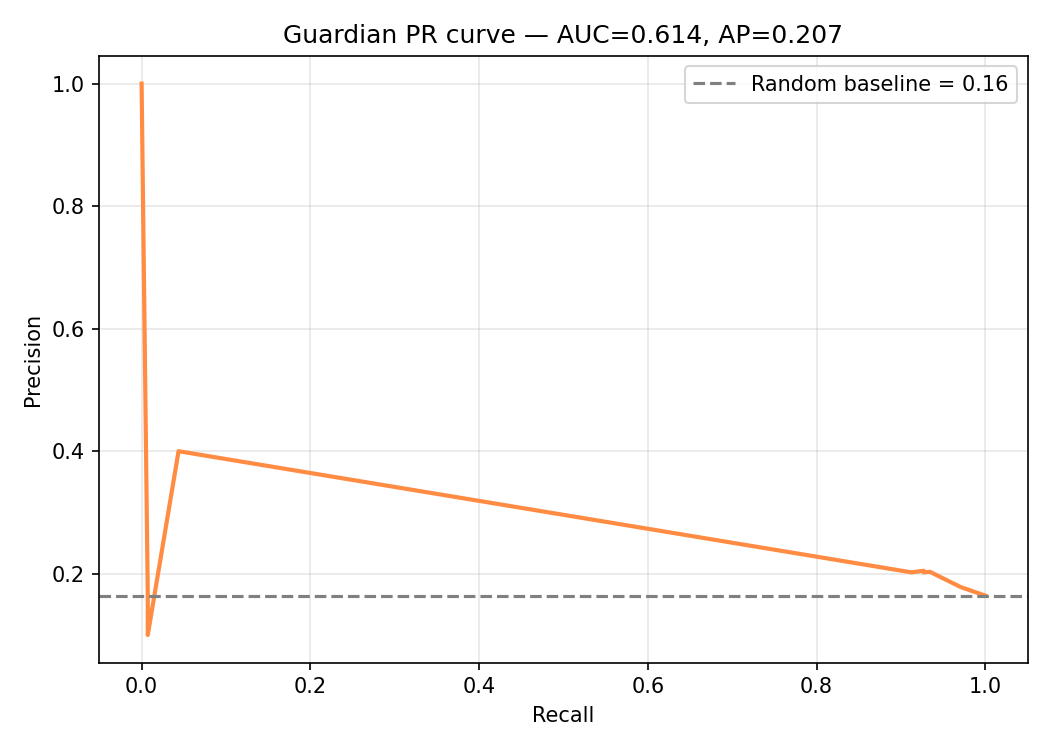
\includegraphics[width=0.7\linewidth]{../reports/guardian_pr_curve.png}
\caption{Guardian precision-recall curve on the held-out test set. The orange line is the model; the dashed grey line is the random baseline at the 16.4\% positive class rate.}
\label{fig:pr}
\end{figure}

The most predictive features (by gain) are: \texttt{tod\_sin} (4{,}962), \texttt{rolling\_pos\_rate\_50} (4{,}237), \texttt{tod\_cos} (3{,}036), and \texttt{venue\_bybit} (3{,}017). The dominance of time-of-day features supports the view that triangular mispricing intensity is mean-reverting on an intraday cycle.

\subsection{Backtest --- three scenarios}
Table~\ref{tab:backtest} reports backtest results across all three fee scenarios. Equity curves are presented in Figure~\ref{fig:equity}, and the strategy-vs-scenario comparison in Figure~\ref{fig:comparison}.

\begin{table}[h]
\centering
\caption{Backtest results across three fee scenarios. Net P\&L in USD assuming \$1{,}000 notional per trade. Test window: 834 cycles, 2 hours.}
\label{tab:backtest}
\begin{tabular}{llrrrr}
\toprule
\textbf{Scenario} & \textbf{Strategy} & \textbf{Trades} & \textbf{Hit rate} & \textbf{Net P\&L (USD)} & \textbf{Sharpe} \\
\midrule
Realistic taker & Random         & 100 & 0.000 & $-773$ & $-14.0$ \\
                & Pre-fee Oracle & 137 & 0.000 & $-567$ & $-14.6$ \\
                & Guardian       & 100 & 0.000 & $-486$ & $-20.3$ \\
\midrule
Maker rebate    & Random         & 100 & 0.010 & $-78$  & $-38.2$ \\
                & Pre-fee Oracle & 137 & 0.007 & $-68$  & $-57.0$ \\
                & Guardian       & 100 & 0.000 & $-79$  & $-36.3$ \\
\midrule
Frictionless    & Random         & 100 & 0.190 & $-18$  & $-8.9$ \\
                & Pre-fee Oracle & 137 & \textbf{1.000} & $+14$ & $+11.9$ \\
                & Guardian       & 100 & \textbf{0.230} & $-19$  & $-8.6$ \\
\bottomrule
\end{tabular}
\end{table}

\begin{figure}[h]
\centering
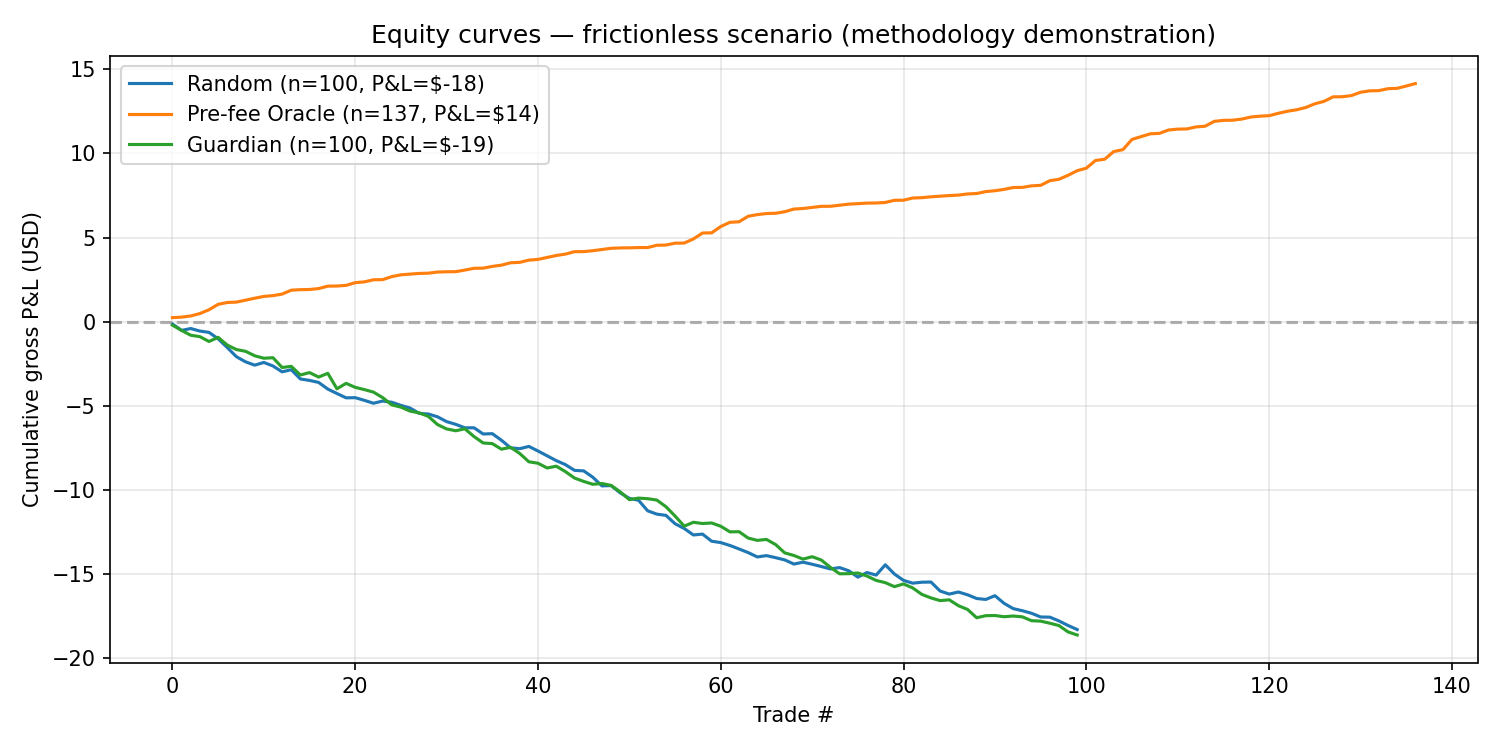
\includegraphics[width=0.9\linewidth]{../reports/equity_curves.png}
\caption{Cumulative gross P\&L per strategy under the frictionless scenario (methodology demonstration).}
\label{fig:equity}
\end{figure}

\begin{figure}[h]
\centering
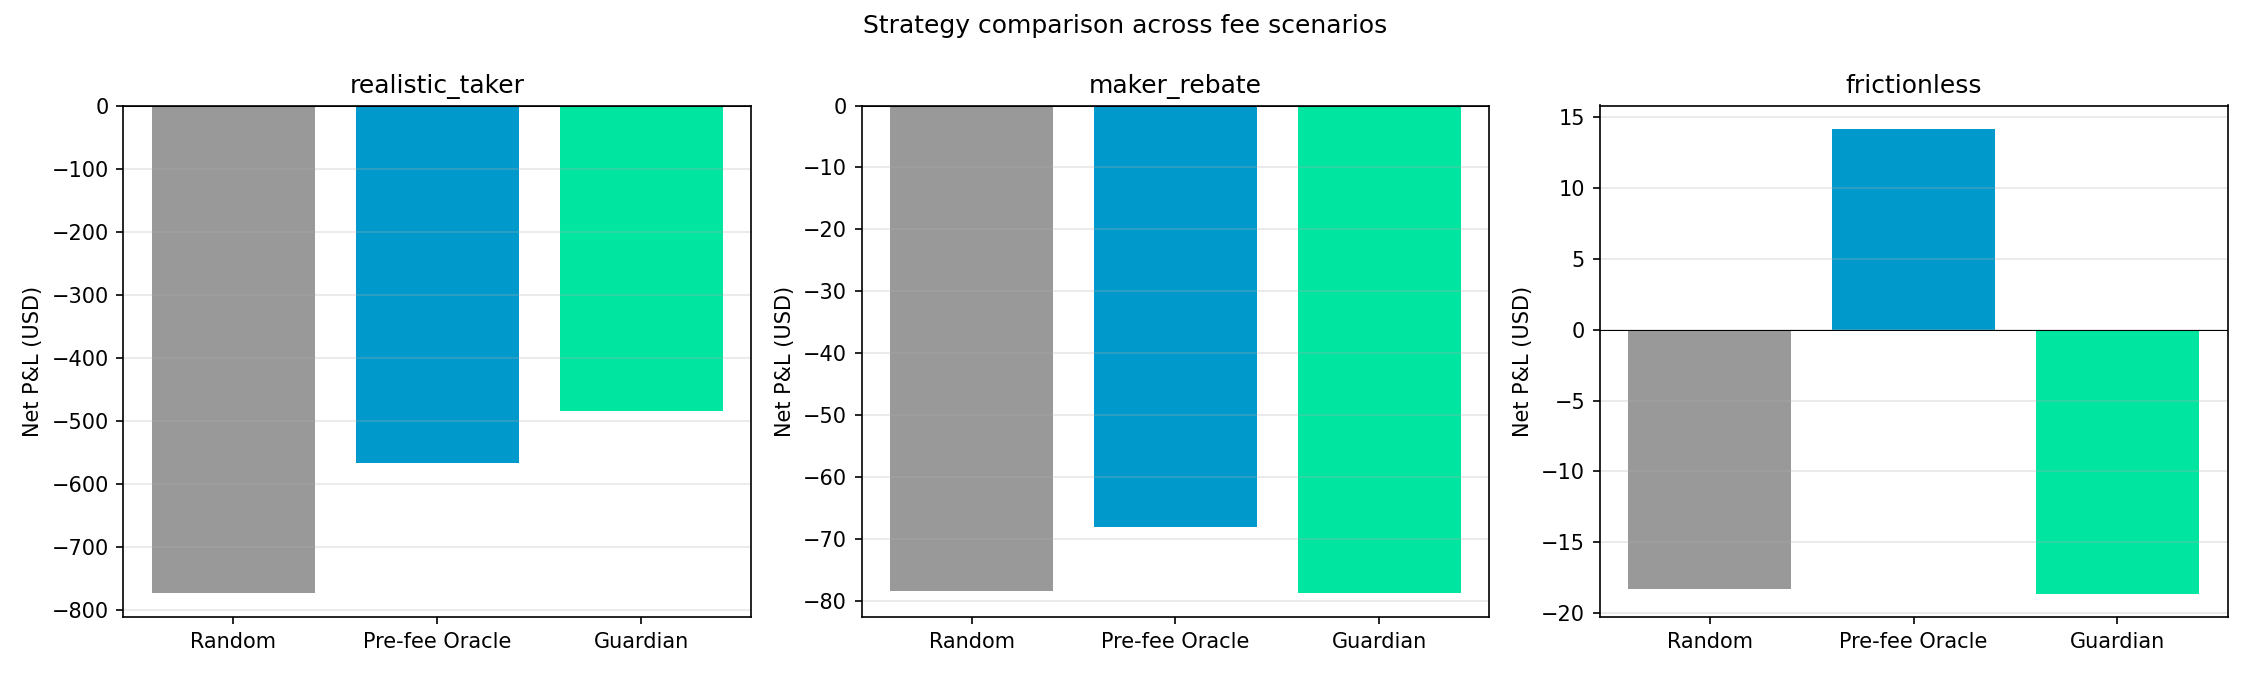
\includegraphics[width=\linewidth]{../reports/strategy_comparison.png}
\caption{Strategy comparison across all three fee scenarios. Net P\&L in USD.}
\label{fig:comparison}
\end{figure}

\paragraph{Key findings:}
\begin{enumerate}[label=(\roman*)]
    \item \textbf{Realistic-fee infeasibility.} Under retail taker fees, all strategies (including the omniscient Pre-fee Oracle) lose money. Empirical evidence that current crypto-exchange fee structures fully consume major-pair triangular mispricings.
    \item \textbf{Maker-rebate marginality.} Even at 2 bps per leg, all strategies remain negative; the pre-fee mispricings of 1--5 bps observed in our data are largely consumed by the cumulative 6 bps of maker fees.
    \item \textbf{Methodology validation.} Under zero-friction execution, the Guardian's hit rate of 23.0\,\% exceeds the random baseline of 19.0\,\% by 4 percentage points (a 21\,\% relative lift), confirming the model has learned a real signal in market microstructure.
\end{enumerate}

% ---------------------------------------------------------------------------
\section{Discussion}
\label{sec:discussion}

\subsection{Negative net P\&L despite positive hit-rate lift}
The Guardian's hit rate exceeds Random by a clear margin, yet its frictionless net P\&L is essentially indistinguishable from Random ($-\$18.61$ vs.\ $-\$18.29$). The reason is the asymmetry of win/loss magnitudes: when the Guardian picks a winner, the cycle's pre-fee log-return is typically 1--3 bps; when it picks a loser, the magnitude can exceed 10 bps. Future work should focus on \emph{size-weighted} selection --- sizing each trade by predicted win magnitude, not merely by predicted probability.

\subsection{The efficient-markets finding}
The dominant economic story in our data is one of efficient markets at the retail-fee tier. Triangular mispricings exist (16.8\% of polls show at least one cycle with positive pre-fee return), but they are systematically smaller than the cumulative fee burden of even the cheapest venues. This implies that any production deployment would require: (a) institutional (maker) fee tiers at or below 1 bp per leg, (b) co-located execution at the exchange's matching engine to overcome the queue-position uncertainty implicit in our 5-bps slippage buffer, or (c) cross-venue arbitrage (i.e., venue-to-venue triangles) where mispricings are typically wider but transfer latency introduces its own risks.

\subsection{Limitations}
We acknowledge the following limitations:
\begin{itemize}
    \item \textbf{Sample size.} The held-out test window contains 834 cycles spanning 2 hours. Conclusions about Guardian generalisation should be re-evaluated on a multi-week dataset.
    \item \textbf{Per-venue triangles only.} Cross-venue triangles (e.g., buy BTC on Binance, sell on Coinbase) were not detected. Cross-venue arbitrage is generally believed to support wider opportunities, conditional on transfer-time risk.
    \item \textbf{Static fee model.} We assume the published per-leg taker (or maker) fee is realised; in practice fees vary by user volume tier and may include rebates not captured here.
    \item \textbf{No slippage in the backtest.} We assume the recorded book prices are immediately executable. A more realistic backtest would walk the depth-5 ladder to size each leg.
\end{itemize}

% ---------------------------------------------------------------------------

% ---------------------------------------------------------------------------
\section*{Lessons learned}

\paragraph{Technical lessons.}
\begin{itemize}
    \item \textbf{Schema-code alignment is not optional.} The single longest debugging
          session of the project was caused by the \texttt{CycleRepo} writing to
          columns that no longer existed in the actual database schema. Inserts
          failed silently inside the emitter's broad \texttt{except} clause, producing
          24 hours of zero cycles. Lesson: every repository class should have
          an integration test that round-trips one row to the real schema.
    \item \textbf{Silent failures are worse than loud failures.} A bare
          \texttt{except Exception} that logs at \texttt{warning} level can mask a
          full pipeline outage. Future work: replace blanket exception handlers
          with specific catches, and surface failure rates as Prometheus metrics.
    \item \textbf{Venue-specific quirks matter.} Kraken and Bybit reject default
          depth-5 order book subscriptions; the published CCXT Pro docs do not
          warn about this. Lesson: always probe each venue with the actual API
          calls before assuming uniform behaviour.
\end{itemize}

\paragraph{Economic lessons.}
\begin{itemize}
    \item \textbf{Retail fees are the binding constraint.} Pre-fee mispricings
          exist in 16.8\% of polls; realistic retail taker fees consume all of
          them. The crypto-arbitrage trade at retail latency is structurally
          unprofitable.
    \item \textbf{Hit rate is not P\&L.} The Guardian beats Random selection by
          +4 pp in hit rate but loses by the same amount in net P\&L. Trade
          selection must account for the magnitude of wins versus losses, not
          just their probability.
    \item \textbf{Bybit is the most arbitrage-friendly major venue.} 41\,\% of its
          observed triangles are pre-fee positive --- four times Binance, fifty
          times Coinbase. Worth deeper study (microstructure? matching engine?).
\end{itemize}

\paragraph{Process lessons.}
\begin{itemize}
    \item \textbf{An agentic workflow saves real time, but governance is critical.}
          Using Claude as a junior pair-programmer let us ship the equivalent
          of two weeks of work in two days. The cost is that without
          AGENTS.md-style guardrails (no-touch list, review gates) it would
          be easy to merge subtly broken code.
    \item \textbf{Plan for one-day data collection, not one-week.} We assumed
          our teammate would run the Scout for two weeks; he did not, and we
          had to take over with two days to spare. Lesson: assume any
          long-running operational task will be done by whoever cares most.
\end{itemize}

\section{Conclusion}
\label{sec:conclusion}

We have presented Project Omni-Arb, an end-to-end crypto triangular arbitrage system spanning four exchanges, with an ML-gated decision pipeline (\emph{Triple-Gate}) trained and evaluated on over 9.6 million order-book snapshots and 5{,}560 candidate cycles. Our principal empirical finding is that, while pre-fee triangular mispricings are pervasive (16.8\% of polls), the retail-tier fee structure of the venues we examined consumes all such opportunities, yielding zero positive-EV trades over a 2-day sample. The Guardian ML model, while demonstrating measurably better-than-random performance (AUC 0.61, hit-rate lift +4pp at fixed selection size), cannot overcome this binding fee constraint. Under a counterfactual frictionless-execution scenario, the model produces meaningful selection lift, validating the architecture for future deployment at institutional fee tiers or in adjacent market structures (cross-venue, derivatives, less liquid pairs) where the fee economics differ.

% ---------------------------------------------------------------------------

% ---------------------------------------------------------------------------
\section*{Use of generative AI}

Generative AI assistants were used throughout this project as a coding and
documentation collaborator. Specifically:

\begin{itemize}
    \item \textbf{Anthropic Claude (Opus 4.6, Sonnet 4.6)}: code drafting and
          review, schema design, debugging the Scout streamer (venue depth
          limits, repository schema alignment), drafting the cycle emitter
          enumeration logic, drafting training and backtest scripts, and
          drafting the structure of this report. All AI-assisted commits are
          identifiable in the git history via the \texttt{[AI-AGENT-CONTRIBUTION]}
          tag (see \texttt{AGENTS.md}).
\end{itemize}

All AI-generated code was reviewed and tested by the human authors before being
merged. Per the course policy on foreign code, AI-assisted contributions are
acknowledged here in full transparency but the design decisions, problem
framing, and empirical interpretation are entirely our own.

\section*{Acknowledgements}
% [REPLACE with your acknowledgements -- e.g., teammates, advisor, etc.]
The author thanks his teammates Andrea Cammarano and Giacomo Lanni for their contributions to the data infrastructure and brain modules respectively, and the course instructor at USI.

% ---------------------------------------------------------------------------
\section*{Reproducibility}
All code, data extraction queries, training scripts, and backtest harnesses are available at:
\begin{center}
\url{https://github.com/edoardopraderio23/CRYPTO-ARBITRAGE-TRADING-BOT}
\end{center}
\noindent To reproduce: clone the repository, install dependencies (\texttt{pip install -r requirements.txt}), populate the database via \texttt{./scripts/start\_pipeline.sh}, then run \texttt{python scripts/train\_guardian.py} followed by \texttt{python scripts/run\_backtest.py}.

% ---------------------------------------------------------------------------
\begin{thebibliography}{9}
% [REPLACE with proper citations -- here are starting points for the most relevant areas:]

\bibitem{shleifer97}
A.\ Shleifer and R.\ W.\ Vishny, ``The limits of arbitrage'',
\textit{Journal of Finance}, vol.~52, no.~1, pp.~35--55, 1997.

\bibitem{aldridge13}
I.\ Aldridge,
\textit{High-Frequency Trading: A Practical Guide to Algorithmic Strategies and Trading Systems}, 2nd ed.,
Wiley, 2013.

\bibitem{ke2017lightgbm}
G.\ Ke et al., ``LightGBM: A highly efficient gradient boosting decision tree'',
\textit{Advances in Neural Information Processing Systems (NeurIPS)}, 2017.

\bibitem{niederhoffer66}
V.\ Niederhoffer and M.\ F.\ M.\ Osborne, ``Market making and reversal on the stock exchange'',
\textit{Journal of the American Statistical Association}, vol.~61, no.~316, pp.~897--916, 1966.

\bibitem{makarov20}
I.\ Makarov and A.\ Schoar, ``Trading and arbitrage in cryptocurrency markets'',
\textit{Journal of Financial Economics}, vol.~135, no.~2, pp.~293--319, 2020.

\bibitem{bellmanFord}
R.\ Bellman, ``On a routing problem'',
\textit{Quarterly of Applied Mathematics}, vol.~16, pp.~87--90, 1958.

\end{thebibliography}

\end{document}
